\usepackage[utf8]{inputenc}
\usepackage[UKenglish]{babel}

\usepackage{amsmath}
\usepackage{amsthm}
\usepackage{amsfonts}
\usepackage{amssymb}

\newtheorem{theorem}{Theorem}
\newtheorem{lemma}{Lemma}
\newtheorem{corollary}{Corollary}
\newtheorem{definition}{Definition}
\newtheorem{example}{Example}

% Thomas packages

\usepackage{algorithm}
\usepackage[noend]{algpseudocode}
\usepackage{enumitem}
\usepackage{multicol}
\usepackage{hyperref}
\usepackage{cleveref}
\let\globcount\newcount % https://tex.stackexchange.com/questions/285950/package-autonum-needs-the-obsolete-etex-package
\usepackage{autonum}
\DeclareMathAlphabet{\mathpzc}{OT1}{pzc}{m}{it}

\DeclareMathOperator{\poly}{poly}
\DeclareMathOperator{\sign}{sign}
\DeclareMathOperator{\asvec}{vec}
\DeclareMathOperator*{\argmax}{arg\,max}
\DeclareMathOperator*{\argmin}{arg\,min}
% Allow page break in align
\allowdisplaybreaks


\usepackage{mathtools}
\DeclarePairedDelimiterX{\infdivx}[2]{(}{)}{#1 \,\delimsize\|\, #2}
\DeclareMathOperator*{\Div}{D}
\newcommand{\D}{\Div\infdivx}
\DeclareMathOperator*{\smallDiv}{d}
\newcommand{\di}{\smallDiv\infdivx}
\DeclareMathOperator*{\h}{h}

% Jakob packages
\newcommand{\eps}{\varepsilon}
\newcommand{\R}{\mathbb{R}}
\newcommand{\Z}{\mathbb{Z}}

\newcommand{\abs}[1]{\left\lvert #1\right\rvert}
\newcommand{\set}[1]{\left\{ #1 \right\}}
\newcommand{\setbuilder}[2]{\left\{ #1 \; \middle\vert \; #2 \right\}}
\newcommand{\norm}[2]{\left\| #1 \right\|_{#2}}
\newcommand{\innerprod}[2]{\left\langle #1, \; #2 \right\rangle}

\newcommand{\Prp}[1]{\Pr\!\left[#1 \right]}
\newcommand{\Prpcond}[2]{\Pr\!\left[#1 \; \middle| \; #2 \right]}
\DeclareMathOperator*{\Ep}{E}
\newcommand{\Epcond}[2]{\text{E}\!\left[#1 \; \middle| \; #2 \right]}

\newcommand{\br}[1]{\left( #1 \right)}


\newcommand{\smat}[1]{\left[\begin{smallmatrix}#1\end{smallmatrix}\right]}
\newcommand{\svec}[1]{[\begin{smallmatrix}#1\end{smallmatrix}]}



\begin{document}


%\title{Getting More from MinHash}
\title{Improved MinHash Estimation for Nearest Neighbor Search}
\author{Thomas Dybdahl Ahle}
\maketitle

\abstract{
   Broder'97~\cite{broder1997resemblance} introduced the idea of Minwise Hashing, which maps a set to a single element in such a way that two significantly overlapping sets are likely to map to the same element.

   Concretely the hash function $h:2^U\to U$ is such that $\Pr[h(X)=h(Y)]=\text{J}(X,Y)$, where $J(X,Y)=\frac{|X\cap Y|}{|X\cup Y|}$ is known as the Jaccard Similarity.

   We introduce a new way to estimate the similarity $J(X,Y)$ given $h(Y)$ and $X$, that is asymptotically optimal in information theoretical terms, and which in practice reduces the number of samples needed by 30\% for a given recall.


   We save a factor of $>1.42$ in variance over the standard method,
   which means a $16\%$ saving in the necessary number of MinHash samples for equivalent confidence bounds.
   In the case of asymmetric set sizes and large similarities the improvement is particularly good, and we show an experimental improvement in recall on standard binary datasets.
}

\section{Introduction}
In the case of search for sets, we'll have a database of minhashes, but a query that's a set.
The question is whether we can do better than simply minhashing the query as well.
Potentially reducing the number of minhash values needed for a given accuracy.

Sometimes MinHash is used for all pairs comparison (many-many), such as in Mash~\cite{ondov2016mash},
but other times we just need to compare with one set (one-many).
In those cases we can save.

Formally, let $x,y$ be any subsets of $[n]$ with $|x\cap y|=v$.
Sample $k$ independent uniform hash functions $h_i : [n] \to [0,1]$.
Define $m_i = \argmin_{z\in y} h_i(z) \in [n]$ to be the $k$ minhash values.

The goal is, given $x$, $(m_i)_{i\in[k]}$ and $|y|$, to estimate $v$ as well as possible.

\begin{figure}[h]
   \centering
   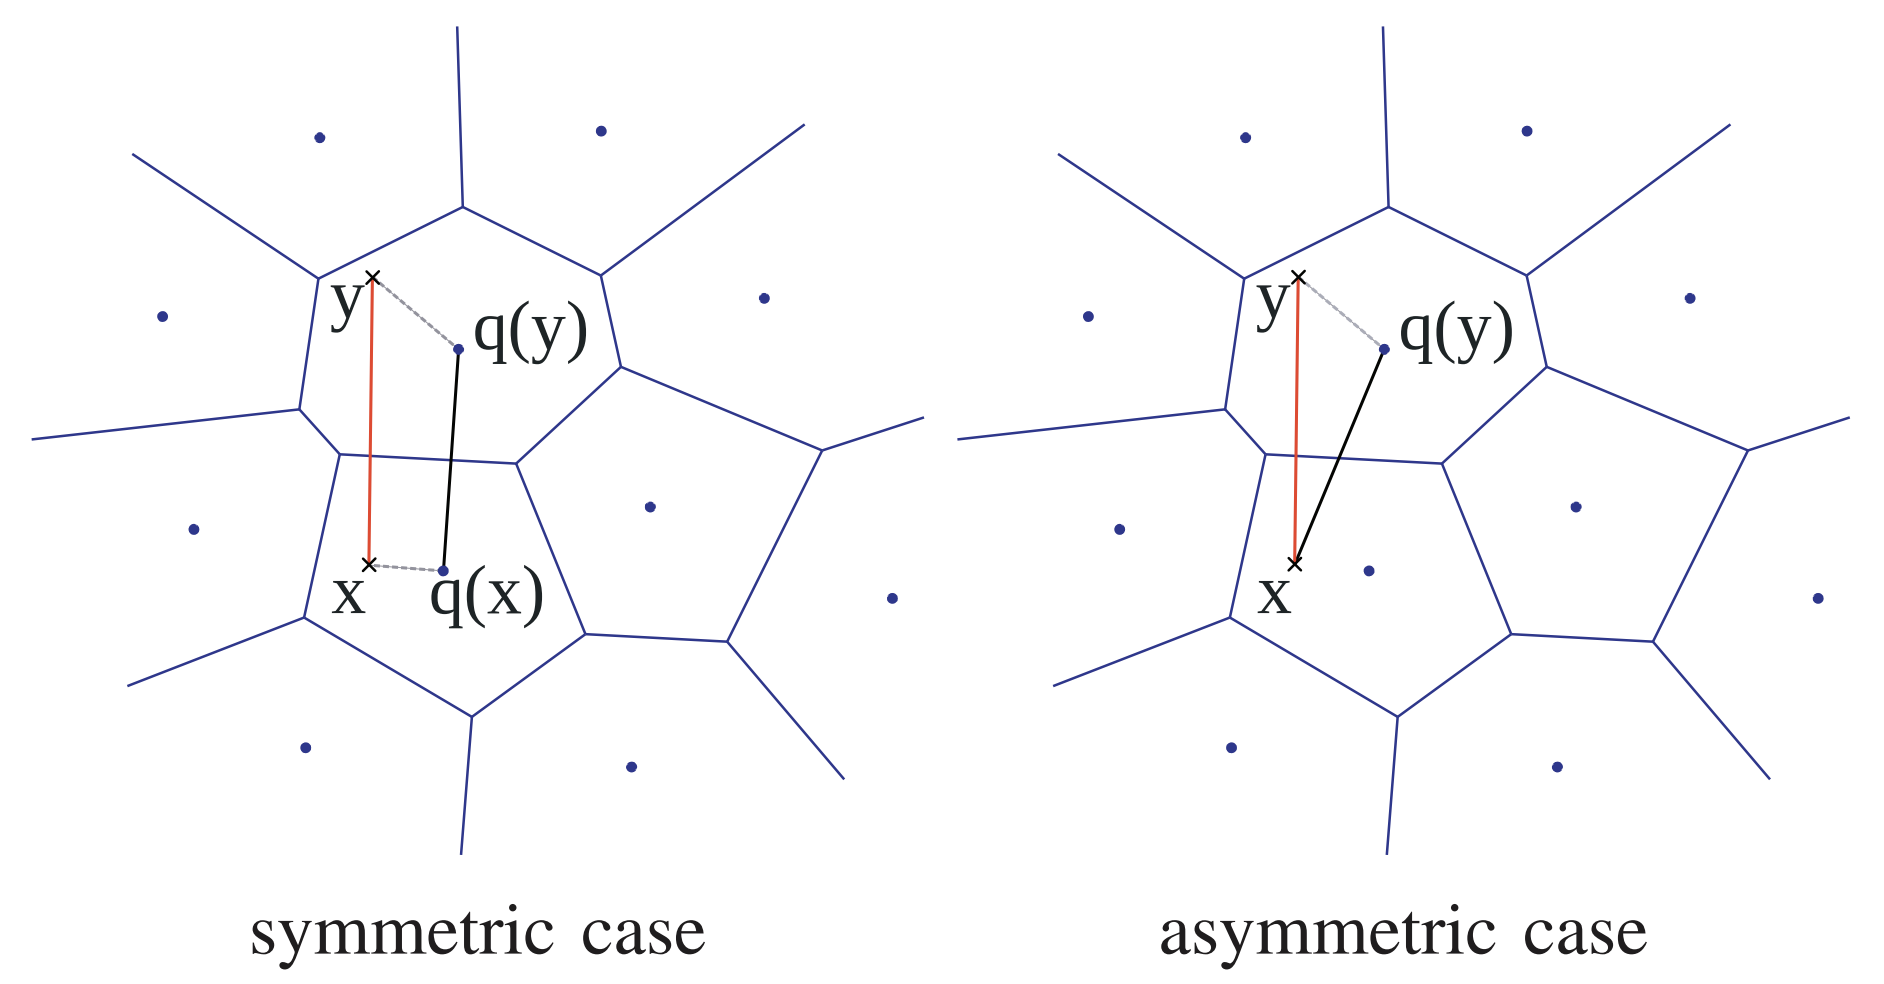
\includegraphics[width=8cm]{figures/pq}
\caption{Figure from~\cite{jegou2010product} illustrating the difference between symmetric and asymmetric estimation, as used in Nearest Neighbor Search.
%For Euclidean distance the idea is quite natural. For MinHash it is harder to do.
}
\end{figure}

\subsection{Related work}

Relation to PQ/AQ.

Pioneerede by~\cite{jegou2010product} 

Relation to one-way communication complexity.

ScaNN~\cite{guo2020accelerating} showed that efficient quantization is key to making the fastest possible data structures.

Product Quantization for Nearest Neighbor Search


KDD 2019: A Memory-Efficient Sketch Method for Estimating High Similarities in Streaming Sets
(Max Log Hash)

TKDE 2018 A Review for Weighted MinHash Algorithms
(How does my method relate to weighted minhash?)

Hyperloglog

SetSketch: Filling the Gap between MinHash and HyperLogLog

B-Bit minhash
Memory wise we can get similar improvements by storing the hash values rather than the indicies(?) And compress them.

Bottom-k minhash

\section{Maximum Likelihood and Cramer Rao}

We start from the lower bound side by considering the Cramer Rao bound with $k=1$.
We define a random variable $Z$ to $\inf$ if $m\not\in x$ and $
= \sum_{z\in x\setminus y} [h(z) \le h(m)]$ otherwise.

Note that we can change the distribution of $h$ to be anything monotone without changing the probabilities.
We'll now assume it has exponential distribution.
%(Also note that that $\log 1/h(z)$ has exponential distribution.)
let $h^* = h(m)$, then $h^* = \min_{z\in y}h(z) \sim \text{Exp}(y)$ by stability of minimums.
We define $p=\Pr[h(z)\le h^*] = 1-\exp(-h^*)$.
Conditioning on $h^*$ we see that $Z$ has binomial distribution $B(n,p)$ where $n=|x\setminus y|$.

Back to the lower bound, 
Cramer Rao asks us to define
\[
   I(j) = E_{z,p}\left[\left(\frac{d\ell(z,p;\; j)}{d\ell}\right)^2\right]
\]
where (for $z\not=\inf$)
\begin{align}
   \exp(\ell(z;j))
   &=\Pr[Z=z]
 \\&= \Pr[m\in x]E_{h^*}[\binom{n}{z}p^z(1-p)^{n-z}]
 \\&= \tfrac{v}{y}E_{h^*}[\binom{n}{z} (1-e^{-h^*})^z e^{-h^*(n-z)}]
 \\&= \frac{v}{n+y}\binom{n}{z}\bigg/\binom{n+y-1}{z}
\end{align}
Approximating
\[
   \binom{n}{z}p^z(1-p)^{n-z} \sim \exp(-n D(z/n, p))
\]


TODO: Can we show that $Z$ is a sufficient statistic?
That is, we don't throw away any information about $v$ by only focusing on $z$ and the sizes of $x$ and $y$.

Actually, I do know $m$, so I also know $h^*$ and $p$.
Maybe that makes things easier?

We get the MLE estimate from the equation $\frac{d}{dj}l(z,p;j)=0$
which reduces to
\[
   \log1/(1-p) = \frac1v\log1/(1-z/(x-v))
\]
Giving a rough estimate of
\[
   v = \log1/(1-p) = \frac1v\log1/(1-z/(x-v))
\]

\subsection{Try two}

Let's assume all the hash values on $x$ are fixed in advance.
Now we pick the values for $y\setminus x$.
We set $m=\argmin_{y_i\in y} h(y_i)$.
We are interested in the probability that $m\in x$ and $m=m^*$ for some element $m^*\in x\cap y$.
We define $h^*=h(m^*)$.

Let $Z$ be the minimum hash value in $y\setminus x$. Then it has distribution $\text{Exp}(|y|-v)$.
We are going to have $m=m^*$ exactly when $Z$ is larger than $h^*$.
(Such that no other value ``wins'' in $y$)
We also need $m$ to be the smallest in $x\cap y$, but that is implied by $m\in x$, since the hash values in $x$ are fixed.
Now $\Pr[Z \ge h^*] = \exp(h^*(|y|-v))$
so the total probability is $\frac{v}{y}\exp(-h^*(|y|-v))$.
This suggest the MLE of $v=-1/h^*$.
That can't be..

Maybe that whole combination argument is wrong.
Surely once we have $\Pr[Z\ge h^*]$ we already have $m\in x$, so we don't actually have that factor $v/y$...

What if I also use information when $m\not\in x$?
I can still compute the hash value of $m$ and compare it to my own hash values...
If $m\not\in x$ we have $Z < h^*$, where again $h^*$ is the smallest hash value in $x\cap y$.
This happens with probability $1-\exp(-h^*(|y|-v))$ which is most likely at $v=0$.
So this suggests a ``bang bang'' estimator, simply dependent on whether $m\in x$.
This is however still different from the normal minhash estimator, which also asks for the value to be smallest in $x$.

At least in my initial experiment, this actually improves recall @ 10!

Men det er selvfølgelig lidt nemt.
Det er der måske ikke noget at gøre ved.

Er det en unbiased estimator?
Nok ikke..
Forventningsværdien er vel $v/y$?
Husk at Jaccard $v/(x+y-v)\le \min\{x,y\}/\max\{x,y\}$ altid.
Så forventningsværdien bliver $\frac{v\min\{x,y\}}{y\max\{x,y\}}$.
På mit lille testset giver det en stor forbedring i recall.

Men vi kan gøre det bedre endnu. For når der er mere end een værdi bliver sandsynligheden jo noget ala
\[
   \prod_i \begin{cases} 1-\exp(-h_i(y-v)) & \text{if } m_i \not\in x \\
   \exp(-h_i(y-v)) & \text{if } m_i \in x \end{cases}
\]
Taking logs and differentiating we have
\[
   \sum_{m_i\in x}{h_i}
   = \sum_{m_i\not\in x}\frac{h_i}{e^{h_i(y-v)}-1}.
\]
which is at least a convex function, so probably reasonably easy to optimize?
However, can we maybe get it on a closed form?

Even better, it seems the rhs is an increasing function in $v$
And we can series / inverse series expand it at $v=0$ to get a good approximation at least for small $v$.

Does the expectation perhaps depend on the $h_i$ values of $x$?
I suppose...
It should be $e^{-h^*(y-v)}$
where $h^*$ is the smallest value in the intersection.

\section{Try 3}

What if we take the permutation view?
We consider the permutation known and not actually random.
But that allows us to consider the choice of $y\setminus x$ and $y\cap x$ as chosen (without replacement) at random.

If $y$ hashes to $m$, it means that $m$ is the left most element of $y$ chosen.
That means $m$ is chosen, and none of the elements to the left.

Case 1: Let's say $m\in x$.
Let $k$ be the number of elements of $x$ to the left of $m$.
Ways to choose all other elements of $x\cap y$ starting from $m$: $x-k-1\choose v$
Ways to choose disjoint elements: $u-m-(x-k)\choose y-v$.
Total ways to choose $y$: $\binom{u-x}{y-v}\binom{x}{v}$.
So the probability is something like
\begin{align}
\frac{\binom{x-k}{v}\binom{u-m-(x-k)}{y-v}}{\binom{x}{v}\binom{u-x}{y-v}}
&\approx
(1-k/x)^v(1-(m-k)/(u-x))^{y-v}
\\&\approx
\exp(-kv/x -(m-k)(y-v)/(u-x))
\end{align}
Again, the log likelihood is monotone in $v$ for a single sample.
But for multiple samples it probably won't be\dots
Hm. If We're just adding linear log likelihoods like the above, it will be...

The likelihood being increasing depends on whether $m/u\ge k/x$, which at least has nice units.

Being more precise, we get a slope of
\[
   (m/u - k/x )/(1 - x/u) - 1/(y - v)
\]
Since the second term is always negative, this says that when $m/u\le k/x$ the slope is negative and the maximum likelihood is at $v=0$.
Otherwise we get $v=y-\frac{1-x/u}{m/u-k/x}$

This approximation seems bad.
It's better to use entropy.
Then we have
\begin{align}
\frac{\binom{x-k}{v}\binom{u-m-1-(x-k)}{y-v-1}}{\binom{x}{v}\binom{u-x}{y-v}}
&= \frac{\binom{x-k}{v}\binom{u-m-(x-k)}{y-v}}{\binom{x}{v}\binom{u-x}{y-v}}\frac{y-v}{u-m-(x-k)}
\\&\approx e^{
   (x-k)H(\frac{v}{x-k})
   -x H(\frac{v}{x})
   +(u-m-x+k)H(\frac{y-v}{u-m-x+k})
   -(u-x) H(\frac{y-v}{u-x})}
\end{align}
\begin{align}
\frac{\binom{x-k-1}{v-1}\binom{u-m-1-(x-k-1)}{y-v}}{\binom{x}{v}\binom{u-x}{y-v}}
&= \frac{\binom{x-k}{v}\binom{u-m-(x-k)}{y-v}}{\binom{x}{v}\binom{u-x}{y-v}}\frac{v}{x-k}
\end{align}

Differentiating we have the slope
\[
   \log\left(\frac{1-k/(x-v)}{1-(m-k)/(u-x-y+v)}\right) - \frac{1}{y-v}
\]
when $m\not\in x$ and 
\[
   \log\left(\frac{1-k/(x-v)}{1-(m-k)/(u-x-y+v)}\right) - \frac{1}{v}
\]
otherwise.

When the sets are much larger than $m$ and $k$,
the $\log$ can be approximated as 
\[
k/(x-v) - (m-k)/(u-x-y+v)
\]

Actually it seems we should just perform the entropy approximation directly, without pulling out the -1s. Then we get slopes of

Differentiating we have the slope
\[
   \log\left(\frac{(1-1/(y-v))(1-k/(x-v))}{1-(m-k)/(u-x-y+v)}\right)
\]
when $m\not\in x$ and 
\[
   \log\left(\frac{1-k/(x-v)}{(1-1/v)(1-(m-k)/(u-x-y+v))}\right)
\]
otherwise.
The other nice thing being that we can actually solve this.
Even if it is a second degree equation.

When $u$ is very big, as is usually the case, these simplify nicely to
\[
   \begin{cases}
      \log\left[(1-\frac{k}{x-v})(1-\frac1{y-v})\right]
      & \text{if } m\not\in x
      \\
      \log\left[\frac{1-k/(x-v)}{1-1/v}\right]
      & \text{if } m\in x
   \end{cases}
\]
and these can be solved to yield respectively
$v = x/(k+1) + (y-1)k/(k+1)$ and $v=x/(k+1)$.
Isn't it weird that we estimate $v$ larger when $m\not\in x$?

The thing is that the first slope is always negative.
We can see that, since
\[
   \frac{d}{dv}\log\left[(1-\frac{k}{x-v})(1-\frac1{y-v})\right]
   = \frac1{1-(y-v)} + \frac1{y-v} - \frac{k}{(x-v)(x-v-k)}.
\]
Elementarily we have $\frac{1}{1-z}+\frac{1}{z} < 0$ for all $z > 0$,
so the first term is always negative.
The second term is negative as well, since $v \le x-k$.
Thus we get the estimate
\[
   v = 
   \begin{cases}
      0 & \text{if } m\not\in x \\
      \frac{x}{k+1} & \text{if } m\in x
   \end{cases}
   .
\]

It might make more sense to estimate $m\approx u/y$ or as a constant times $u$, but then we still end up with a second order equation.

I also like the approximation $(m-k)/(u-x-y+v) \approx m/u$ and $k/(x-v)\approx k/x$.
That gives the equations
\[
   v = 
   \begin{cases}
      y + \frac{1-k/x}{k/x-m/u} & \text{if } m\not\in x \\
      \frac{1-m/u}{k/x - m/u} & \text{if } m\in x
   \end{cases}
   .
\]

My idea for estimating the full MLE estimator is the following:

Differentiating we have the slope
\begin{align}
   &\frac{1}{n}\sum_i \begin{cases}
      \log\left(\frac{(1-1/(y-v))(1-k_i/(x-v))}{1-(m_i-k_i)/(u-x-y+v)}\right)
      &\text{when $m_i\not\in x$}
      \\
   \log\left(\frac{1-k_i/(x-v)}{(1-1/v)(1-(m_i-k_i)/(u-x-y+v))}\right)
      &\text{when $m_i\in x$}
   \end{cases}
   \\&=
      \log\left(\frac{
         (1-1/(y-v))^{n_2/n}
         (\prod_i(1-k_i/(x-v)))^{1/n}
      }{
         (1-1/v)^{n_1/n}
         (\prod_i (1-(m_i-k_i)/(u-x-y+v)))^{1/n}
      }\right)
   \\&\approx
      \log\left(\frac{
            (1-\frac{n_2/n}{y-v})
            (1-\frac{\sum_i k_i/n}{x-v})
      }{
         (1-\frac{n_1/n}{v})
         (1-\frac{(\sum_i m_i-k_i)/n}{u-x-y+v})
      }\right)
\end{align}
which we can set equal to 0 quite easily.
The division by $n$ seems a bit magical to me.
Without it the approximation isn't as good, and may not even be defined.
But then why not just set $n\to\infty$?
That actually gives the comb2 method.
So maybe we should just use that...
Probably there is some accuracy trade-off with some optimal division factor.

Another thing: There may still be some cases where there is no solution within the acceptable range.
I should probably do something about that?


It's fun to note we are back to one of the very first estimators we made.

We should try and recall the bias estimates we made back then.
Maybe the arguments actually made sense after all?


\begin{align}
   \frac{d}{dv}\ell(m,k;v)&=
   \log\left(\frac{(1-\frac1{y-v})^{[m\not\in x]}(1-\frac{k}{x-v})}{(1-\frac 1v)^{[m\in x]}(1-\frac{m-k}{u-x-y+v})}\right)
   \\
   I(v) = \frac{d^2}{dv^2}\ell(m,k;v)&=
    [m\not\in x](\frac1{y-v}-\frac1{y-v-1})
   + (\frac1{x-v}-\frac1{x-v-k})
                            \\&
   +[m\in x](\frac1v-\frac1{v-1})
   + (\frac1{u-x-y+v}-\frac1{u-x-y+v-m+k})
\end{align}
This feels like something we could potentially take the expectation over and get a Cramer Rao lower bound...
The $[m\not\in x]$ and $[m\in x]$ terms are easy.
So it's just a matter of taking
$E\frac1{x-v-k}$ and $E\frac1{u-x-y+v-m+k}$.
That seems like something that could be pushed into the binomial coefficients..

The problem is that the expectation depends on the hash values of $x$ in new ways (other than just through $k$ and $[m\in x]$.
I suppose we want to take the expectation over the $x$ hash values as well.
This is justified by the fact, that for the actual estimator, we want to take into account all the information we have available.
However for the analysis, we don't have any information of how the xs will hash.
%We could also do it over the worst case $x

Maybe it's easier if we lower bound by $\frac{1}{x-v-k+1}$, since then we don't run into troubles at $k=x-v$ and we have e.g.
\[
   \sum_k\frac1{x-v-k+1}\binom{x-k}{v}\bigg/\binom{x}{v} = \frac{x+1}{v(x-v+1)}
\]
Using
\begin{align}
   \frac1{x-v-k+1}\binom{x-k}{v}
   &=
   \frac1{x-v-k+1}\binom{x-k}{x-v-k}
 \\&=
   \frac1{x-k+1}\binom{x-k+1}{x-v-k+1}
 \\&=
   \frac1{x-k+1}\binom{x-k+1}{v}
 \\&=
   \frac1{v}\binom{x-k}{v-1}
\end{align}
So also
\[
   \sum_k \frac1v\binom{x-k}{v-1}\binom{u-m-x+k}{y-v}
   = \frac1v\binom{u-m+1}{y}
\]

Mathematica also seems to think it is reasonably easy to sum
\[
   \sum_k\frac1{x-v-k+1}\binom{x-k-1}{v-1}\bigg = \frac{x-1}{(x-v)(v-1)}\binom{x-2}{v-1}
\]

\section{Estimators}

A key approximation for fast estimation, is the following estimator:
\[
   \min\left\{\frac{bx}{b+k}, by\right\}.
\]
We arrive at this by considering two cases of the approximate MLE equation.
To get some intuition to why this is a good estimator, we note that
\[
   E\left[by\right] = v.
\]
and 
\[
   E\left[\frac1{k+1}\right] = \frac{y}{x-v+1}(H_{x+y-v+1}-H_{y-1})
   \approx \frac{y}{x-v+1}\log\left(\frac{x+y-v+1}{y-1}\right).
\]

\[
   E\left[\frac{bx}{b+k}\right] = \frac{vx}{y}E\left[\frac1{1+k}\right]
\]

and for $|x|=|y|$ large,
\[
   E\left[\frac{b}{b+k}\right] = \frac{2j}{1-j}\log\frac2{1+j} + O(1/|x|) \approx \frac{4j}{3+j}
\]
which is related to the Sørensen–Dice coefficient $\frac{2j}{1+j}$ recently used in the Mash distance for genome distance\footnote{ Ondov, Brian D., et al. "Mash: fast genome and metagenome distance estimation using MinHash." Genome biology 17.1 (2016): 1-14.}
Note however that this expectation is for a single sample, and our estimator uses $b$ 

\[
   E\left[\frac{1}{x-v-k+1}\right] = \frac{y}{(y-1)(x-v+1)}\left(1-\frac{1}{\binom{x+y-v}{y-1}}\right)
\]

\[
   E\left[\frac{1}{u-x-y+v-m+k+1}\right] = \frac1{y-1}
\left(\frac{y}{u-x-y+v+1}-\frac1{\binom{u-x+v}{y}}\right)
\]


\begin{align}
   \frac{d}{dv}\ell(m,k;v)&=
   \log\left(\frac{(1-\frac1{y-v+1})^{[m\not\in x]}(1-\frac{k}{x-v+1})}{(1-\frac 1{v+1})^{[m\in x]}(1-\frac{m-k}{u-x-y+v+1})}\right)
   \\
   = \frac{d^2}{dv^2}\ell(m,k;v)&=
    [m\not\in x](\frac1{y-v+1}-\frac1{y-v})
   + (\frac1{x-v+1}-\frac1{x-v-k+1})
                            \\&
                            +[m\in x](\frac1{v+1}-\frac1{v})
   + (\frac1{u-x-y+v+1}-\frac1{u-x-y+v-m+k+1})
   \\
   I(v) = -E[\frac{d^2}{dv^2}\ell(m,k;v)]
   \approx \frac{1}{y(x-v)} + \frac1{v(y-v)}
\end{align}
If $|x|=|y|=n$ that the variance $1/I(v)$ is maximized at $(\sqrt{2}-1)n$ with value $(\sqrt2-1)^2n^2$.
That's cool.

In general wee can get bounds like
\[
   V(X) \in [1-2\sqrt{2}/3, 1/16]\frac{m(4 xy-m^2)}{x},
\]
where $m=\min{x,y\}$,
or (the incomparible) $V(X) \le (\sqrt{2}-1)^2x^{1/2}y^{3/2}$.
It is natural that we have some assymetry between $x$ and $y$, since that's the whole point of this paper.

So what is the equivalent variance with Symmetric Minhash?

Well, we have
$   \Pr[h(x)=h(y)] = j$
Let $Z = [h(x)=h(y)]$, then
$E[Z]=j$.
Now $E[Z^2] =E[Z] = = j$, so $V[Z] = j-j^2=j(1-j)$.

For MLE estimatoren siger vi
\[
   I(j) = I(v)/j'(v)^2
\]

This gives a variance that's always better than that of MinHash.
It is particularly good when $x$ and $y$ are different sizes, but even in the case where they equals it gives a variance of 
\[
   j(1-j)\frac{(1+j)^3}{2(1+3j)}
\]
which is $< 0.1756$, saving a factor $> 1.424$ over MinHash.

\section{Experiments}


Mention stuff about
Use of Stirling's approximation.
Use of Newton's method.

\begin{itemize}
   \item Show plots of how close our approximate estimator is to the "Real" MLE
   \item Show effect on recall
\end{itemize}

\subsection{Recall}

The following shows the effect on recall@10 with 10,000 queries:
\begin{table}[h!]
\centering
 \begin{tabular}{|r| r r r r r|} 
 \hline
 K  &Symmetric & Asym $n=1$ & Asym $n=2$ & Asym $n=4$ & Asym $n=8$ \\
 \hline
 1 & 0.0019 & 0.0035  & 0.0039 & 0.0045 & 0.0043 \\
 10 & 0.0456 & 0.0477 & 0.0462 & 0.0475 & 0.0477\\
 30 & 0.1499 & 0.1821  & 0.1835  & 0.1872 & 0.1888\\
 100 & 0.3885 &  0.4971  & 0.5013 & 0.5023 & 0.5023  \\
 500 & 0.8020 & 0.8662 & 0.8672 & 0.8672 & 0.8672 \\
  \hline
 \end{tabular}
\end{table}

These results use the minhash estimator as the initial guess.
An alternative is to estimate $v$ as $by/K$, since $Eb=v/y$.
However that appears to be worse, giving recall 1@10 of 0.1718 at newton=1 and $K=30$.
With more newton steps, however, the recall "recovers" to 0.1889 at newton=8.
($n=2$ and $n=4$ gives recall 0.1754 and 0.1826 respectively.)

This data is not true, just an example of a table that might be better:
\begin{table}[h!]
\centering
 \begin{tabular}{|r| r r r r r|} 
 \hline
 K  & Symmetric & MLE & Asym & Asym $n=1$ & Asym $n=8$ \\
 \hline
 1 & 0.0019 & 0.0049  & \textbf{0.0057} & 0.0038 & 0.0044 \\
 10 & 0.0456 & 0.0410 & \textbf{0.0628} & 0.0518 & 0.0474 \\
 30 & 0.1499 & 0.1826 & \textbf{0.1948}  & 0.1921 & 0.1887 \\
 100 & 0.3885 &  .  & 0.4732 & 0.4986 & \textbf{0.5022}  \\
 500 & 0.8020 & 0.865\footnote{Run only with $M=1000$ due to time constrains} & 0.8471 & 0.8671 & \textbf{0.8672} \\
  \hline
 \end{tabular}
\end{table}

A nice estimator appears to be $b \min\{y/K, x/(b+k)\}$, which gets 0.1948 even with 0 newton!
We see that MLE is eventually best (as it should be),
but out simple heuristic estimator is very good for small $K$.
For larger $K$ a single Newton iteration seems easily sufficient.

Some timing data:
%Tid for -K 100 --newton 1
%Time preparing: t1=2813.205824613571, Time searching: t2=5754.812134742737
%Tid for -K 100 --newton 2
%Time preparing: t1=2768.65847158432, Time searching: t2=5648.562669038773
%Tid for -K 100 --newton 4
%Time preparing: t1=2715.9863698482513, Time searching: t2=5616.8901562690735
%Tid for -K 100 --newton 8
%Time preparing: t1=2769.066630601883, Time searching: t2=6230.902306318283
%
%-K 1 --newton 8
%Time preparing: t1=31.681596994400024, Time searching: t2=765.3667838573456

\subsection{Estimation}


\begin{figure}[h]
   \centering
   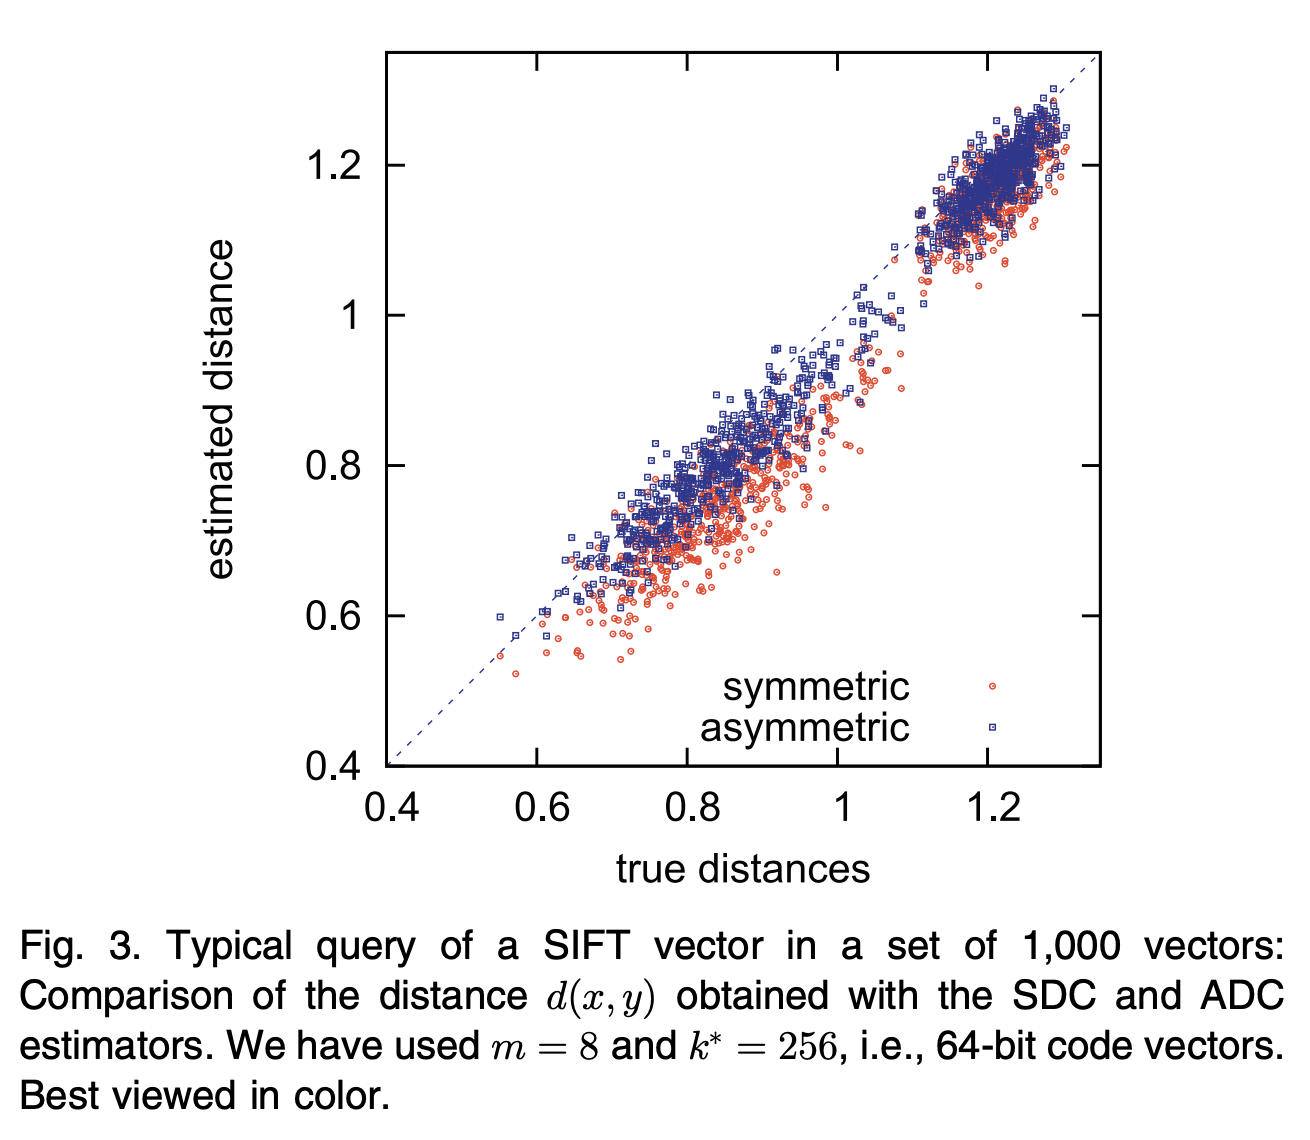
\includegraphics[width=8cm]{figures/estimates}
\caption{It would be nice to have a plot like this as well, showing whether we improve on all scales.}
\end{figure}



\section{Effect of approximation}
From http://galton.uchicago.edu/~eichler/stat24600/Handouts/l02.pdf

If the model is incorrectly specified and the data $Y$ are sampled from a true
density $f^∗$ then the ML estimate converges to the value $\theta∗$ which minimizes
the Kullback-Leibler information
\section{Conclusion}

We have shown that it is possible to substantially improve upon the traditional MinHash estimator in the one-way setting.

\section{Open Problems}

Can we also better estimate other types of MinHash?
\begin{enumerate}
   \item Weighted MinHash
   \item $b$-bit MinHash
   \item Bottom-$k$ MinHash
   \item Find the best sketch for sets in general. Like how Supermajorities is best for queries.
\end{enumerate}


\bibliographystyle{unsrt}
\bibliography{aminhash}

\appendix

\section{Appendix}

\subsection{Nice summation}
Let $n_x=|x|$ and $n_y=|y|$.
For a warm-up we show
\begin{align}
   \sum_{0\le m < u}
   \binom{n_x-k(m)-[m\in x]}{v-[m\in x]}
   \binom{u-m-[m\not\in x]-(n_x-k(m))}{n_y-v-[m\not\in x]}
   = \binom{n_x}{v}\binom{u-n_x}{n_y-v}
   .
\end{align}

We will use the following standard binomial sum:
\begin{align}
   \sum_{a<k<b}\binom{k}{c} &= \binom{b}{c+1} - \binom{a+1}{c+1}
   %\sum_{k=0}^u\binom{k}{c} &= \binom{b+1}{c+1} - \binom{a}{c+1}
\end{align}

Define a sequence $(a_i)_{i\in[0,n_x+1]}$ such that $a_0=-1$, $a_{i+1} = x_i$ for $i\in[n_x]$ and $a_{n_x+1}=u$,
where we see $x$ as a vector in $[u]^{n_x}$.

We consider the sum of terms for the chunk of $m$s between two consecutive $a$ values.
\begin{align}
   &
   %\sum_{0\le k \le n_x}
   \sum_{a_k < m < a_{k+1}}
   \binom{n_x-k}{v}
   \binom{u-m-1-(n_x-k)}{n_y-v-1}
   %+
   %\binom{n_x-k-1}{v-1}
   %\binom{u-a_{k+1}-(n_x-k)}{n_y-v}
   \\&=
   \binom{n_x-k}{v}
   \left[
   \binom{u-a_k-1-(n_x-k)}{n_y-v}
   -
   \binom{u-a_{k+1}-(n_x-k)}{n_y-v}
\right]
   \label{eq:sum_dif}
\end{align}
Define $c_k = \binom{u-a_k-(n_x-k+1)}{n_y-v}$,
We are the interested in the sum
\begin{align}
   \sum_{0\le k \le n_x}
   \binom{n_x-k}{v}(c_k-c_{k+1})
   +
   \sum_{0\le k < n_x}
   \binom{n_x-k-1}{v-1}c_{k+1}
   \label{eq:sum_all}
\end{align}
We substitute $k\mapsto k+1$ in the first term of \eqref{eq:sum_dif} to get the sum
\[
   \binom{n_x}{v}c_0
   +
   \sum_{0 < k+1 \le n_x}
   \binom{n_x-k}{v}
   c_k
   =
   \binom{n_x}{v}c_0
   +
   \sum_{0 \le k < n_x}
   \binom{n_x-k-1}{v}
   c_{k+1}
\]
which we can combine with the second term of \eqref{eq:sum_all}
using the fact that $\binom{n_x-k-1}{v} + \binom{n_x-k-1}{v-1} = \binom{n_x-k}{v}$
to give
\[
   \sum_{0\le k < n_x}
   \binom{n_x-k}{v}
   c_{k+1}
   .
\]
This allows cancellation with the second term of \eqref{eq:sum_dif},
leaving us with
\[
   \binom{n_x}{v}c_0
   -
   \binom{n_x-n_x}{v}c_{n_x+1}
   =
   \binom{n_x}{v}\binom{u+1-(n_x+1)}{n_y-v}
   -
   \binom{0}{v}
   \binom{0}{n_y-v}.
\]
Now $\binom{0}{v}=[v=0]$, so unless $n_y=0$ this second term is 0, leaving us with
$\binom{n_x}{v}\binom{u-n_x}{n_y-v}$.


\end{document}

